
%(BEGIN_QUESTION)
% Copyright 2011, Tony R. Kuphaldt, released under the Creative Commons Attribution License (v 1.0)
% This means you may do almost anything with this work of mine, so long as you give me proper credit

Nuclear reactors generate immense quantities of heat through a phenomenon called {\it nuclear fission}, whereby atoms of a particular substance ``split'' when struck by neutron particle radiation, releasing more neutron particles to split other atoms, and so on in a ``chain reaction''.  Basic control of a fission reactor's power output is achieved by precisely positioning a series of special metal rods called {\it control rods} to absorb excess neutron radiation and thereby regulate the chain-reaction.  Inserting these rods deeper into the reactor core quenches the reaction, while drawing them out of the reactor core increases the reaction.  Instantaneous reactor power output is measured by a set of {\it neutron detectors} located in the core, sensed by a radiation transmitter (RT) and passed on to a control-rod controller (RC).  A process flow diagram (PFD) shows the basic process and neutron flux control loop:

$$\includegraphics[width=15.5cm]{i01752x01.eps}$$

In this case, the reactor uses water as the coolant, pressurized to a level so that boiling is impossible within the reactor vessel.  The heat from the reactor is transferred to a secondary ``loop'' of water by a heat exchanger called a {\it steam generator}.  The secondary water is boiled there, becoming steam to turn a steam turbine to power an electrical generator.  The turbine's exhaust is condensed back into water by another heat exchanger, and then that secondary water is pumped back to the steam generator to be boiled again.

\vskip 10pt

In order to achieve stable and responsive power control as an electricity-generating operation, though, much more instrumentation is needed than what is shown in this PFD.

\filbreak

This PFD shows instrumentation as might be seen on a commercial pressurized-water nuclear power reactor:

$$\includegraphics[width=15.5cm]{i01752x02.eps}$$

Make this diagram even more descriptive by adding the following details:

\begin{itemize}
\item{} Label each input and output signal path for each controller (PV, SP, Out) 
\item{} Sketch arrow-heads to show the direction each control signal path sends information
\item{} Identify the action of each controller (direct vs. reverse), assuming direct-acting transmitters and signal-to-open final control elements
\item{} Identify the ``polarity'' of each input on the summer (i.e. whether each input has a ``+'' or a ``$-$'' symbol next to it describing its proper direction of action
\item{} Identify which controllers have local versus remote (cascade) setpoints
\item{} Identify the feedforward signal path in this control strategy
\end{itemize}

Finally, explain how this control system is supposed to work by conducting at least one ``thought experiment'' whereby the system responds appropriately to some change.

\vskip 20pt \vbox{\hrule \hbox{\strut \vrule{} {\bf Suggestions for Socratic discussion} \vrule} \hrule}

\begin{itemize}
\item{} In most feedforward control strategies, a load signal is added to the manipulated variable signal of a feedback control loop.  In this system, however, we don't see this exact scheme.  Does this still truly qualify as a {\it feedforward} control strategy?  Why or why not?
\item{} Does this control system seek to maintain mass balance, energy balance, or both?
\item{} The primary coolant loop is pressurized by a special device not shown in either PFD, called a {\it pressurizer}.  Research how one of these devices works (your {\it Lessons In Industrial Instrumentation} textbook explains this) and explain it in your own words.
\end{itemize}

\underbar{file i01752}
%(END_QUESTION)





%(BEGIN_ANSWER)

$$\includegraphics[width=15.5cm]{i01752x03.eps}$$

\begin{itemize}
\item{} RC = reverse action
\item{} PIC = direct action (assuming its output goes to the ``$-$'' input on the summer; reverse action would be appropriate if both summer inputs were ``+'')
\item{} FIC = reverse action
\item{} JIC = reverse action
\end{itemize}

The power controller (JIC) and steam pressure controller (PIC) both have local setpoint values.  The neutron flux controller (RC) and flow controller (FIC) are cascade slave units.  

\vskip 10pt

The feedforward signal path is from the power controller (JIC) output to the gain/bias function.  When the power controller calls for more power, it not only cascades an increased setpoint value to the steam flow controller, but it also feeds that information to the neutron flux controller to call for a greater reactor power output.

%(END_ANSWER)





%(BEGIN_NOTES)

The control strategy shown here is based on the feedforward flow/pressure/neutron strategy shown on page 178 of M.A. Schultz's wonderful textbook, {\it Control of Nuclear Reactors and Power Plants} (McGraw-Hill, 1955).

%INDEX% Process: nuclear power reactor control system

%(END_NOTES)


